        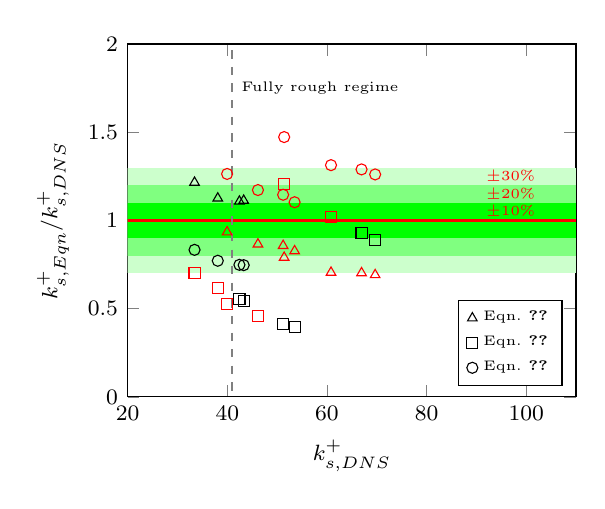
\begin{tikzpicture}[]
        \centering
        \begin{axis}[
            ylabel={$k_{s,\text{Eqn}}^+/k_{s,\text{DNS}}^+$},
            xlabel={$k_{s,\text{DNS}}^+$},
            ymin=0, ymax=2,
			xmax=110,
			xmin=20,
			%xtick={-2,-1.5,...,-0.4},
            width=.6\textwidth,
            height=.5\textwidth,
            label style={font=\footnotesize},
            legend style={font=\tiny,anchor=south east},
                        legend pos=south east,
            tick label style={font=\footnotesize}
            ]
			 \fill[color=green!20,opacity=20] (0,1.3) -- (200,1.3) -- (200,0.7) -- (0,0.7) -- cycle;
			 \fill[color=green!50,opacity=50] (0,1.2) -- (200,1.2) -- (200,0.8) -- (0,0.8) -- cycle;
			 \fill[color=green!100,opacity=100] (0,1.1) -- (200,1.1) -- (200,0.9) -- (0,0.9) -- cycle;

			\addplot [
            black,only marks,mark=triangle,
            ]
            coordinates{
                        (43.2934,48.1821/43.2934)
            (42.4361,47.0239/42.4361)
            (38.0918,42.8840/38.0918)
            (33.4265,40.6182/33.4265)                
            
            };
			\addlegendentry{Eqn.~\ref{Chan2}}
			\addplot [
            black,only marks,mark=square,
            ]
            coordinates{
            (53.5170,21.1/53.5170)
            (51.2133,21.1/51.2133)
            (69.6860,62.0685/69.6860)
            (66.9536,62.0685/66.9536)
                        (43.2934,23.5162/43.2934)
            (42.4361,23.5162/42.4361)
            };
			\addlegendentry{Eqn.~\ref{flack}}
			\addplot [
            black,only marks,mark=o,
            ]
            coordinates{
            (43.2934,32.3208/43.2934)
            (42.4361,31.7575/42.4361)
            (38.0918,29.3891/38.0918)
            (33.4265,27.8554/33.4265)  
            
            };
			\addlegendentry{Eqn.~\ref{forooghi}}
	
	%						\addplot [
         %   black,only marks,mark=star,
         %   ]
         %   coordinates{
         %   (69.69,42.44/69.69)
         %   (66.95,41.60/66.95)
         %   (60.82,33.65/60.82)
         %   (51.42,29.61/51.42)
         %   (53.52,39.17/53.52)
         %   (51.21,38.09/51.21)
         %   (46.15,30.57/46.15)
         %   (39.96,26.58/39.96)
         %   (43.29,39.96/43.29)
         %   (42.44,39.17/42.44)
         %   (38.09,31.19/38.09)
         %   (33.65,27.22/33.65)
         %   };
		%	\addlegendentry{Eqn.~\ref{thakkar}~\cite{Thakkar2017}}
	
	
	
				\addplot [
            red,only marks,mark=triangle,
            ]
            coordinates{
                        (53.5170,44.2578/53.5170)
            (51.2133,43.8871/51.2133)
            (46.1548,39.9460/46.1548)
            (39.9648,37.3339/39.9648)
            
                        (69.6860,48.1821/69.6860)
            (66.9536,47.0239/66.9536)
            (60.8249,42.8840/60.8249)
            (51.4186,40.6182/51.4186)            
            
            };
	
			\addplot [
            red,only marks,mark=square,
            ]
            coordinates{
            (46.1548,21.1/46.1548)
            (39.9648,21.1/39.9648)

            (60.8249,62.0685/60.8249)
            (51.4186,62.0685/51.4186)           

            (38.0918,23.5162/38.0918)
            (33.4265,23.5162/33.4265)  
            };	
			\addplot [
            red,only marks,mark=o,
            ]
            coordinates{
                        (53.5170,59.0430/53.5170)
            (51.2133,58.6687/51.2133)
            (46.1548,54.1087/46.1548)
            (39.9648,50.5004/39.9648)
            
                        (69.6860,87.8597/69.6860)
            (66.9536,86.3284/66.9536)
            (60.8249,79.8904/60.8249)
            (51.4186,75.7211/51.4186)   
            };	
	
	
	
	
	
	
	
	
	
	
	
	
						\addplot [
            red,thick,solid,mark=square,
            ]
            coordinates{
            (0, 1)
            (201, 1)
            };
            						\addplot [
            gray,thick,dashed,mark=square,
            ]
            coordinates{
            (40.9356, 3)
            (40.9356, -1)
            };
			\node[red,right] at (axis cs: 90,1.05) {\tiny $\pm10\%$};
						\node[red,right] at (axis cs: 90,1.15) {\tiny $\pm20\%$};
									\node[red,right] at (axis cs: 90,1.25) {\tiny $\pm30\%$};
																		\node[black,right] at (axis cs: 40.9356,1.75) {\tiny Fully rough regime};
        \end{axis}
        \end{tikzpicture}